\documentclass[10pt,aspectratio=43,mathserif]{beamer}
\usepackage[UTF8]{ctex}
\usepackage{graphicx}
\usetheme{AnnArbor}
\usecolortheme{beaver}
\usepackage{cite}
% Removes icon in bibliography
\setbeamertemplate{bibliography item}[text]

\title{引力的本质}
\subtitle{古典哲学\ 相对论\ 量子理论}
\author{崔家铜 \ 刘润泽\ 朱一中}
\institute{北京航空航天大学物理学院}
\date{2023年12月1日}

\AtBeginSection[]
{
	\begin{frame}<beamer>
	\frametitle{\textbf{目录}}
	\tableofcontents[currentsection]
\end{frame}
}
% \beamerdefaultoverlayspecification{<+->}
% -----------------------------------------
\begin{document}
\frame{\titlepage}
\begin{frame}{目录}
\tableofcontents
\end{frame}

\section{引言}
\begin{frame}{古典物理学}
    % \frametitle{}
    \begin{columns}
        \begin{column}{.3\linewidth}
            \centering
            \begin{figure}[thbp]
                \resizebox{1\linewidth}{!}{
                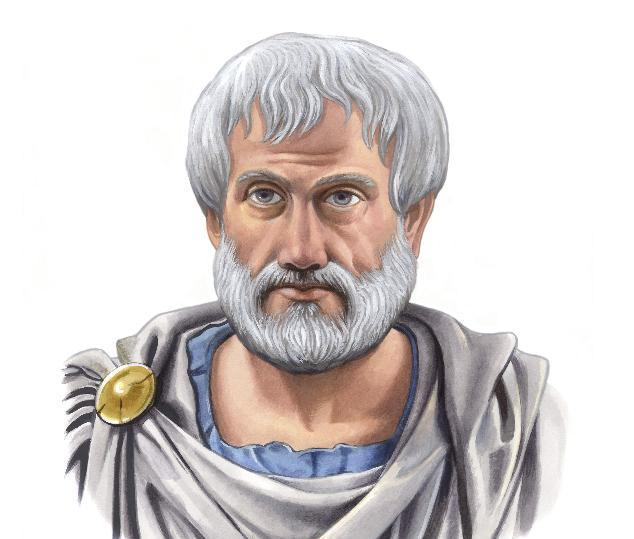
\includegraphics[width=\linewidth]{fig/人物-亚里士多德.jpeg}
                }
                \caption{\footnotesize 亚里士多德(古希腊)}
                \label{fig:ylsdd}
            \end{figure}
        \end{column}
        \hfill
        \begin{column}{.6\linewidth}
            亚里士多德对引力形成了初步的认识
            \begin{enumerate}
                \item 物体总有向着其「正确位置」靠近的趋势
                \item 物体按照其重量的比例向地球的中心坠落
            \end{enumerate}
            此后,伴随天文学的发展,阿尔比鲁尼提出天体具有质量,天体之间也具有引力作用,物体
            受到的引力取决于其与「宇宙中心」的距离\cite{starr2015lost}.
        \end{column}
    \end{columns}
\end{frame}

\begin{frame}{近代对引力的认识}
    \begin{columns}
        \begin{column}{.4\linewidth}
            \centering
            \begin{figure}[htbp]
                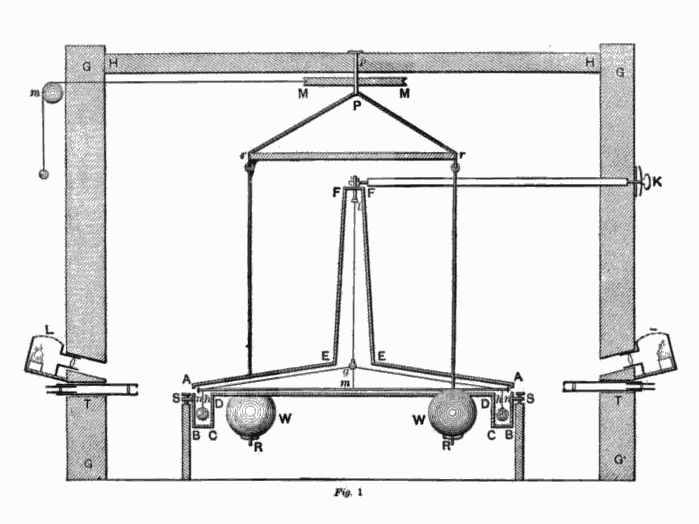
\includegraphics[width=1\linewidth]{fig/Cavendish_Experiment.png}
                \caption{卡文·迪许扭秤}
                \label{fig:niucheng}
            \end{figure}
        \end{column}
    
    \hfill
    \begin{column}{.5\linewidth}
        近代以来,科学家对引力的认识逐渐趋于成熟,承认物体之间有总是存在的相互吸引的相互
        作用,这个力的大小与其距离有关。
        \begin{enumerate}
            \item 哥白尼提出,引力是物体之间的固有相互作用,天体运行依靠引力相互作用
            \item 罗伯特·虎克提出天体重力定律\cite{qadir1989relativity}:$F\propto \frac{1}{r^2}$
            \item 牛顿提出万有引力定律:$F=\frac{Gm_1m_2}{r^2}$\ \footnote{标量式}
            \item 卡文·迪许扭秤实验测得$G=6.74\times 10^{-11} m^3\cdot kg^{-1} \cdot s^{-2}$
        \end{enumerate}
    \end{column}
\end{columns}
\end{frame}
\begin{frame}{现代引力理论}
    现代理论理论主要有广义相对论和经发展的量子引力理论。
    \begin{columns}
        \begin{column}{.4\linewidth}
            \centering
            \begin{figure}[htbp]
                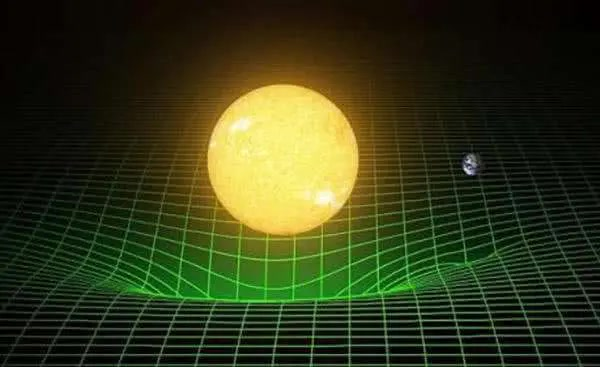
\includegraphics[width=0.8\linewidth]{fig/123.jpg}
                \caption{广义相对论中时空扭曲带来的引力}
                \label{fig:ETgravity1}    
            \end{figure}
        \end{column}
        %\hfill
        \begin{column}{.4\linewidth}
            \centering
            \begin{figure}[htbp]
                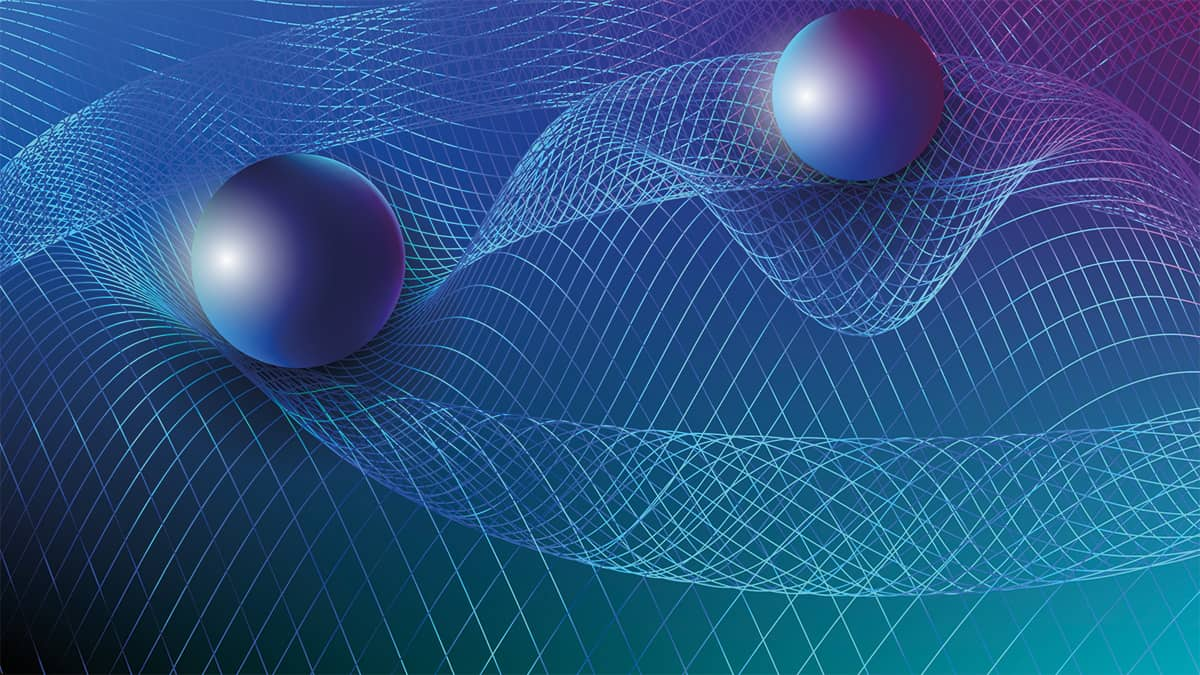
\includegraphics[width=0.8\linewidth]{fig/gravity-and-particles-1754139353-Shutterstock_Evgenia-Fux.jpg}
                \caption{量子重力理论中冷原子之间的引力作用}
                \label{fig:QGtwoAtoms}
            \end{figure}
        \end{column}
        %\hfill
    \end{columns}
\end{frame}

\begin{frame}[allowframebreaks]{References}
	%\bibliographystyle{plain}
	\bibliographystyle{amsalpha}
	%\bibliography{mybeamer} also works
	\bibliography{./mybeamer.bib}
\end{frame}
\end{document}